{
\begin{figure*}[th]
\begin{minipage}{0.50\columnwidth}
\begin{center}
\centerline{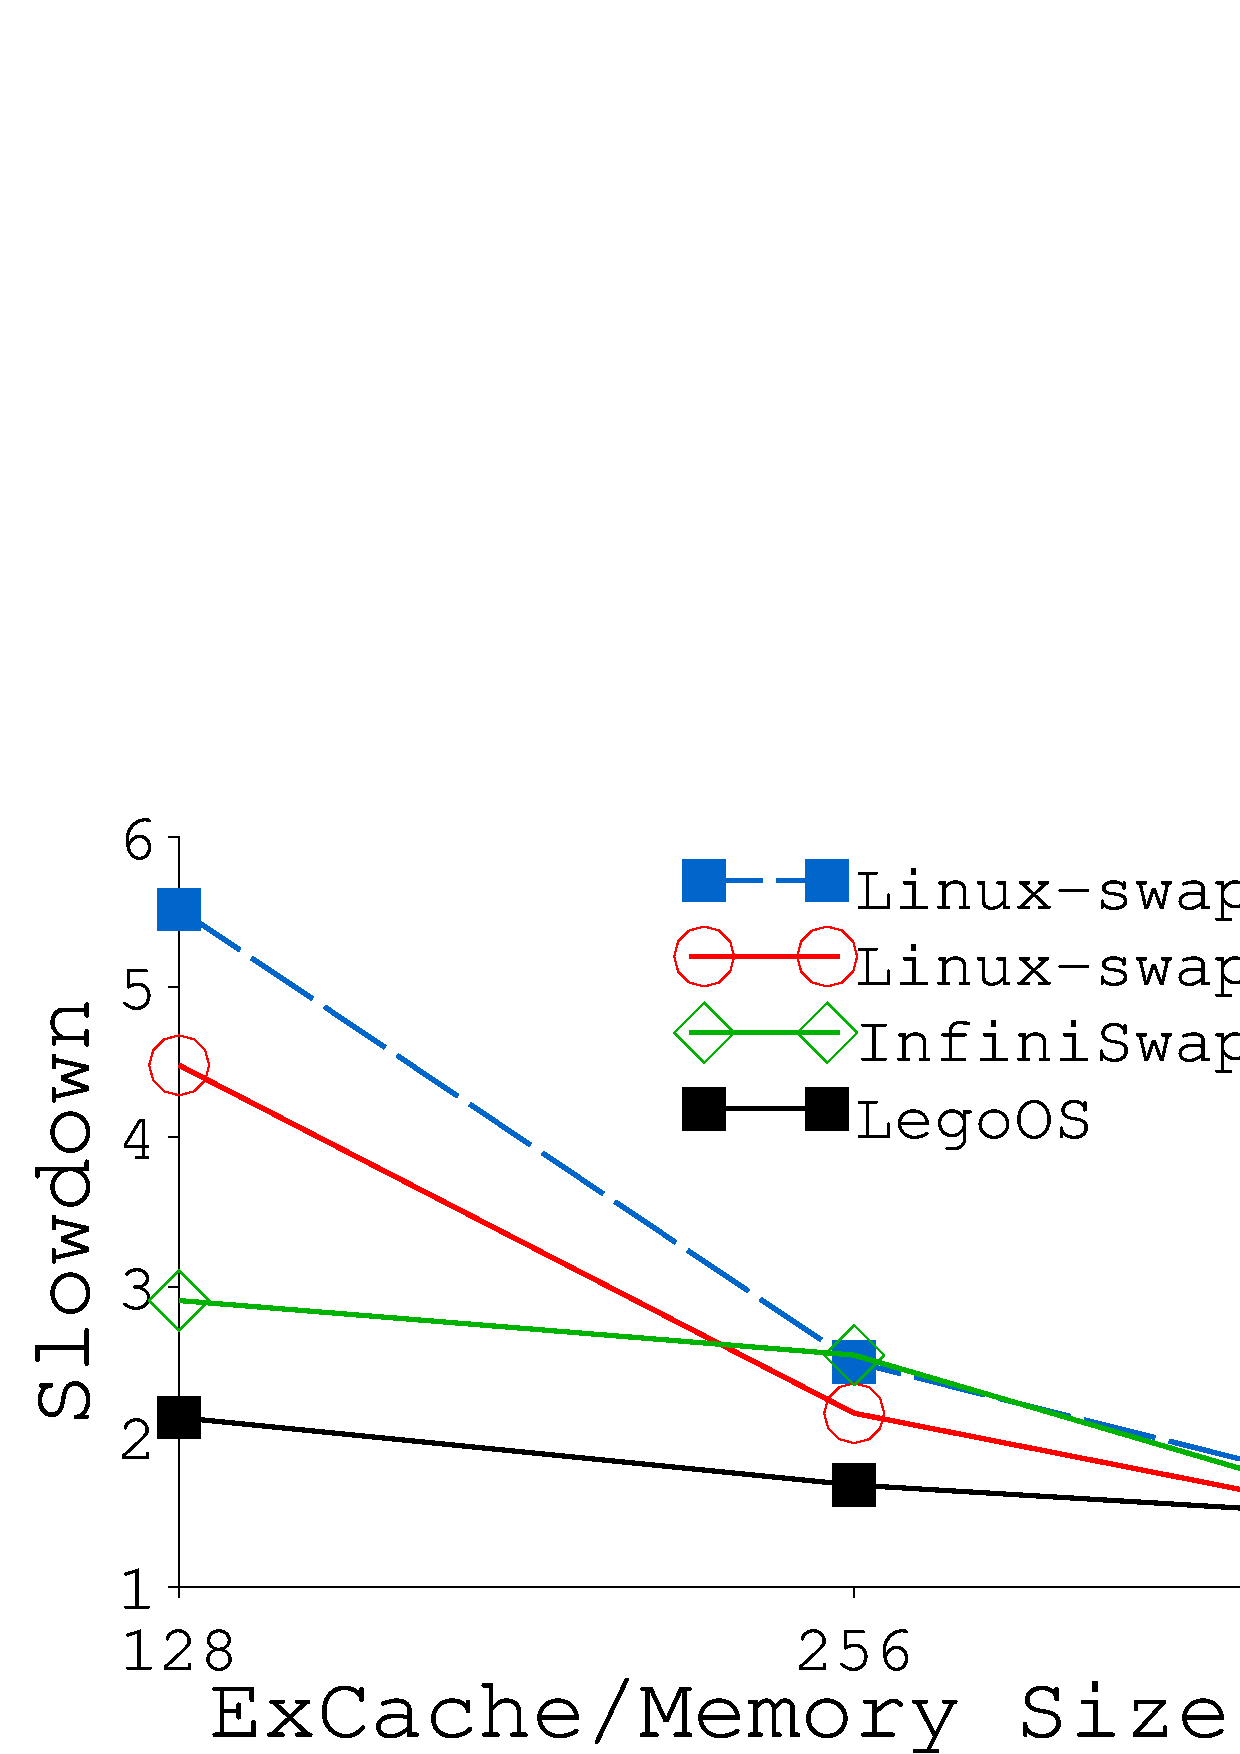
\includegraphics[width=1.0\columnwidth]{Figures/g_plot_LEGO_tf4.pdf}}
\vspace{-0.1in}
\mycaption{fig-tf4}{TensorFlow Perf.}
{
%TensorFlow and Phoenix running on Lego with different ExCache size configurations.
%Compared with running on Linux with limited memory.
}
\end{center}
\end{minipage}
\begin{minipage}{0.50\columnwidth}
\begin{center}
\centerline{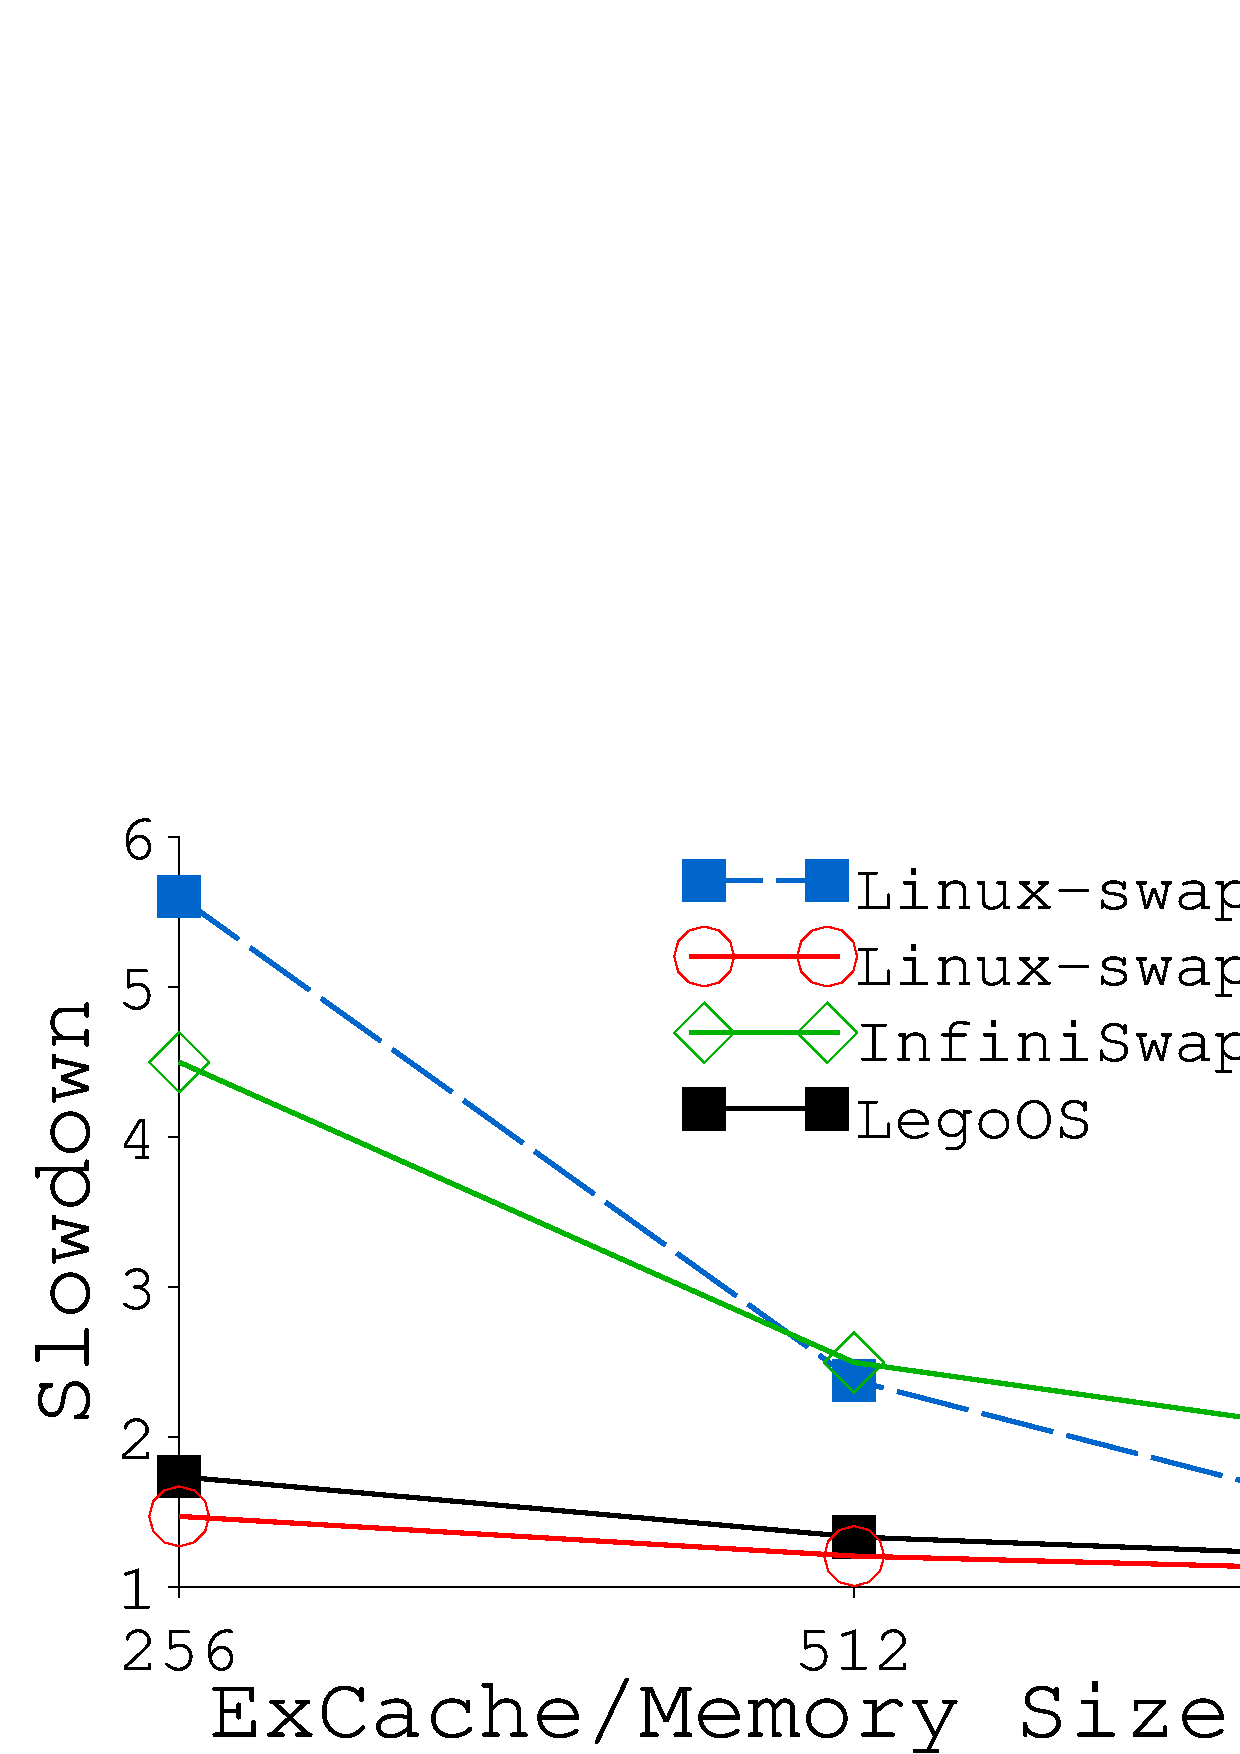
\includegraphics[width=1.0\columnwidth]{Figures/g_plot_LEGO_phoenix.pdf}}
\vspace{-0.1in}
\mycaption{fig-phoenix}{Phoenix Perf.}
{
%TensorFlow and Phoenix running on Lego with different ExCache size configurations.
%Compared with running on Linux with limited memory.
}
\end{center}
\end{minipage}
\begin{minipage}{0.50\columnwidth}
\begin{center}
\centerline{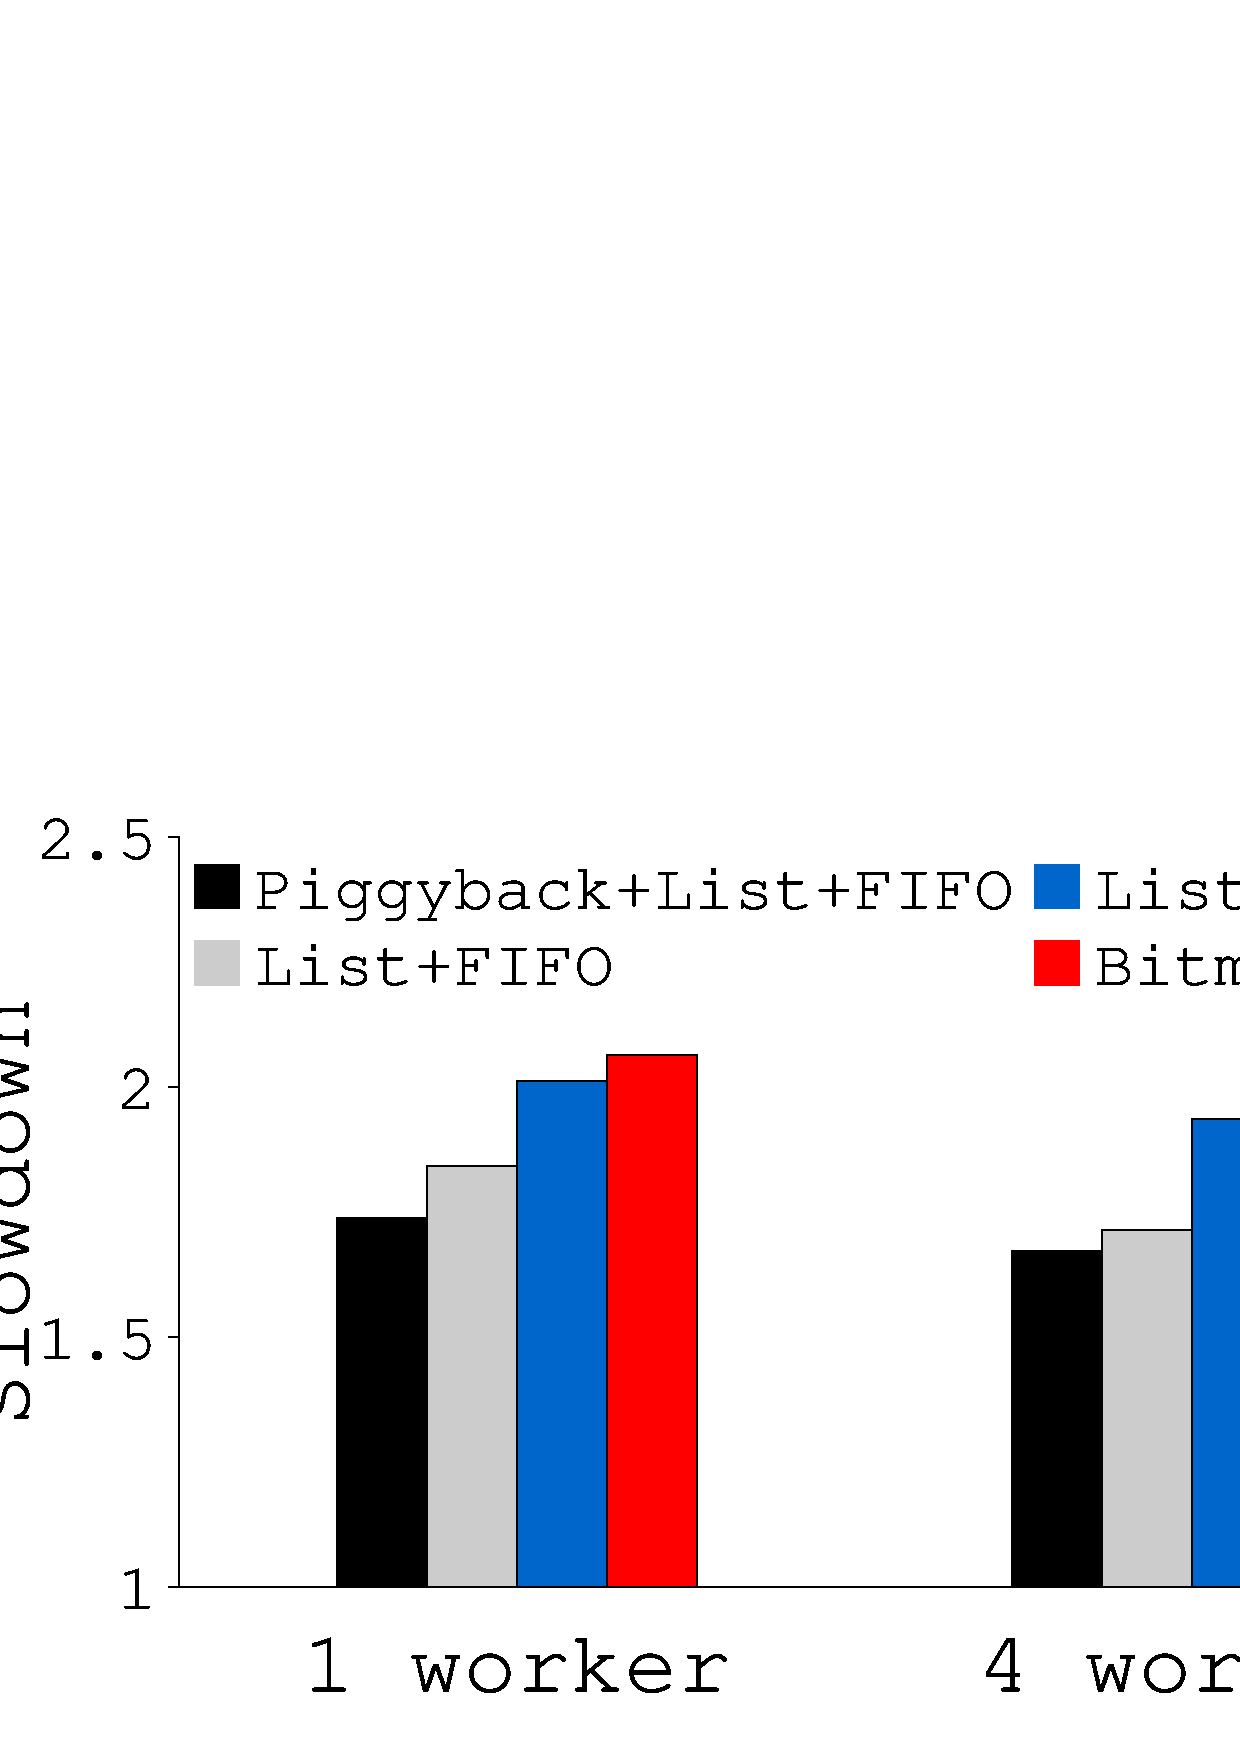
\includegraphics[width=1.0\columnwidth]{Figures/g_plot_LEGO_excache_tech.pdf}}
\vspace{-0.06in}
\mycaption{fig-excache-opt}{ExCache Mgmt.}
{
%TensorFlow and Phoenix running on Lego with different ExCache size configurations.
%Compared with running on Linux with limited memory.
}
\end{center}
\end{minipage}
\begin{minipage}{0.50\columnwidth}
\begin{center}
\centerline{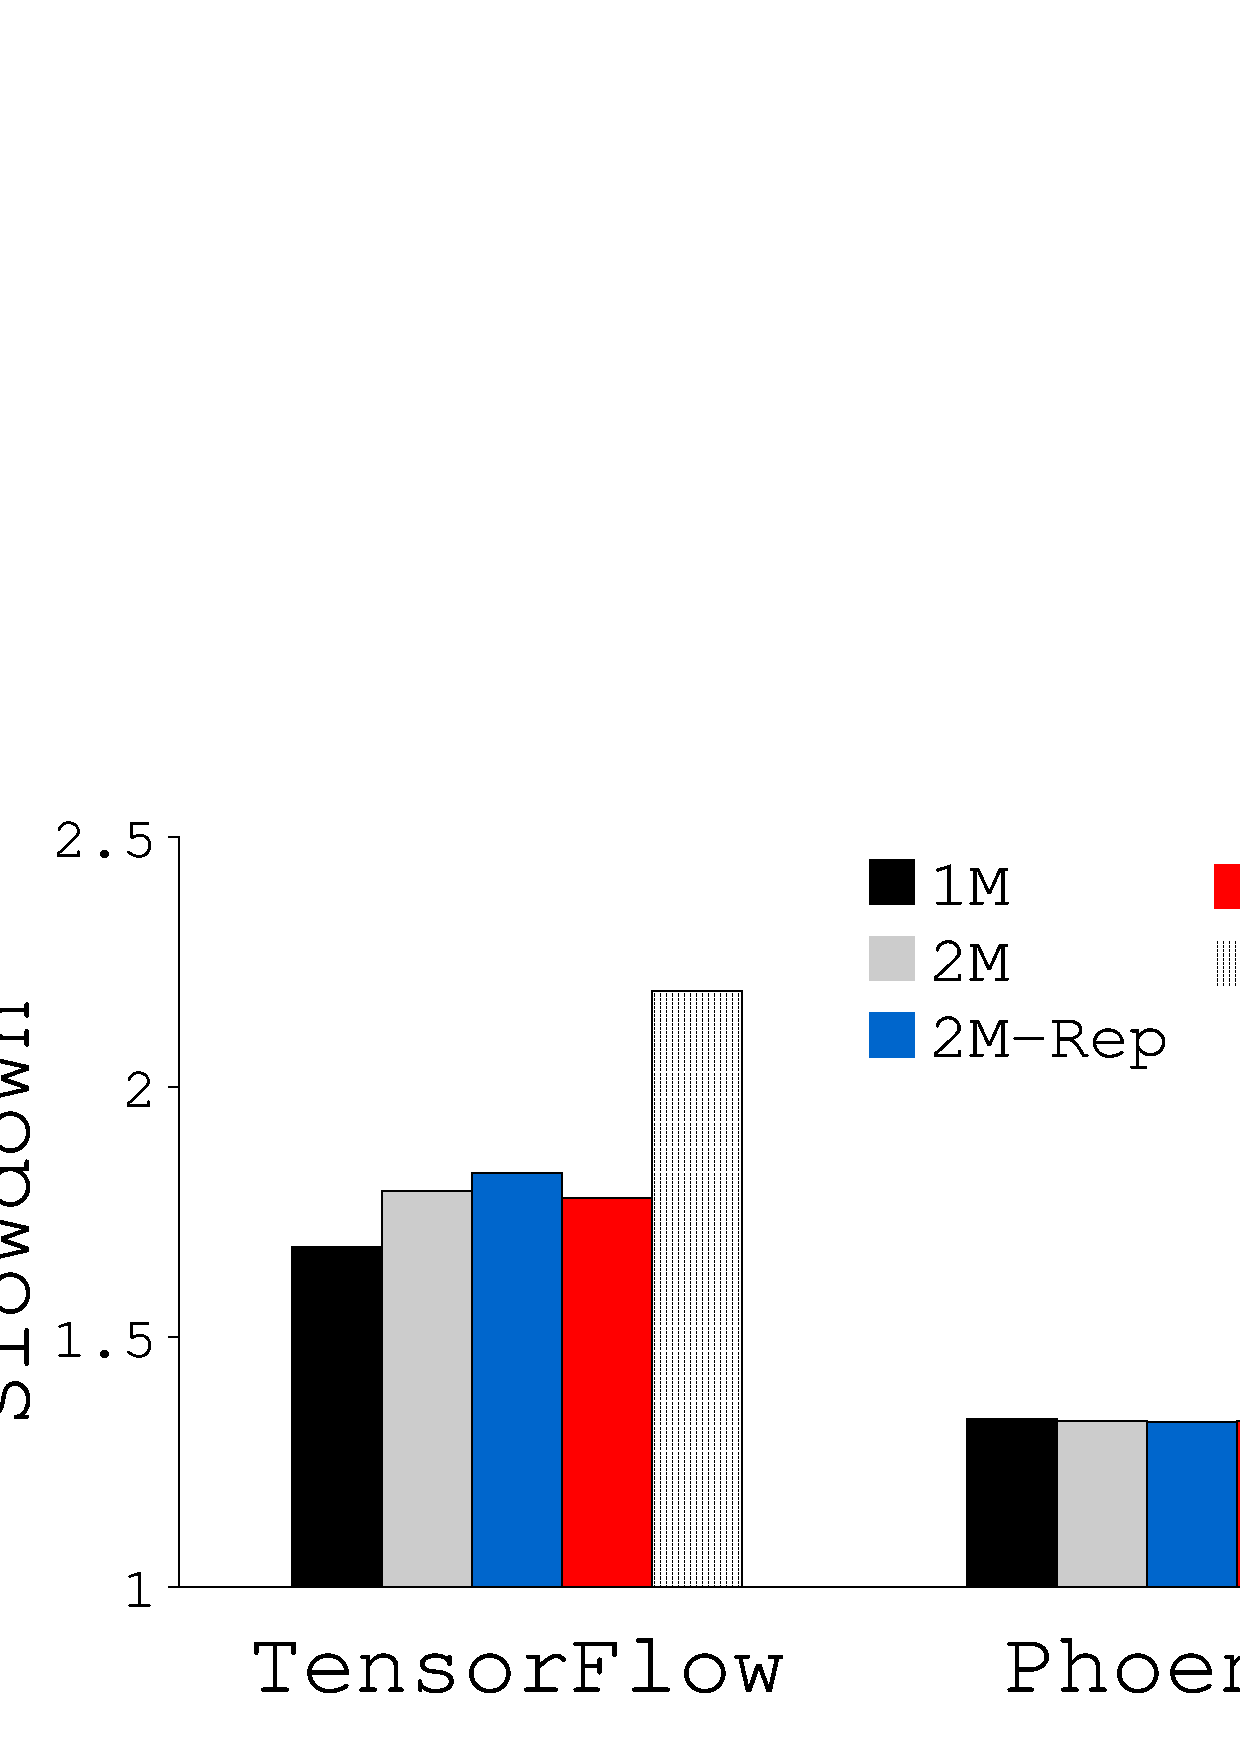
\includegraphics[width=1.0\columnwidth]{Figures/g_plot_LEGO_number_memory_rep.pdf}}
\vspace{-0.06in}
\mycaption{fig-mem-rep}{Memory Config.}
{
%The effect of having multiple memory components and memory replication.
}
\end{center}
\end{minipage}
\vspace{-0.1in}
\end{figure*}
}
